\chapteruaf{Introduction}

Digital systems have become ubiquitous in our society over the past several decades. One of the negative consequences of this change is that these systems are vulnerable to a great number of threats. One method introduced in the past decade to combat this is Virtual Machine Introspection (VMI) which aims to analyze the state of a virtualized Operating System (OS) called a guest. While research into VMI has been extensive ~\cite{bahram_dksm:_2010,pfoh_exploiting_2010,dolan-gavitt_leveraging_2011,dolan-gavitt_virtuoso:_2011,gu_process_2011-1,fu_bridging_2013,garfinkel_virtual_2003,hay_forensics_2008} the security implications of VMI remain largely unexplored. This dissertation will concern itself with the detectability and reliability of VMI.

\section{Computer Security}

The three pillars of computer security are integrity, availability, and confidentiality~\cite{bishop_computer_2012}.  The integrity of a computer system is the property that it will behave as intended by both the user and the designer or programmer.  The availability of a system is the property that a system can be used by a user at any time required. The confidentiality of a system is the property that it can only be accessed by authorized users.  We consider the security of a system to be breeched if any one of these is violated. 

For an example let's consider Gmail [cite gmail].  A user expects that an email sent to their boss will go to their boss. The user also expects the email client will deliver the message exactly as written. These are examples of integrity. A user with an internet connection can access Gmail at anytime day or night. This is an example of availability. In order to access the account and send emails as a specific user or to read his or her emails one must login with a user name and a password.  This is an example of confidentiality of a system. 

A VMI agent can breech the security of a computers system by either attacking the integrity or the confidentiality of that system. The breach of confidentiality can occur when a VMI agent reads the pages of a target system and a breach in the integrity can occur if the VMI agent alters the pages of a target system. 

\section{Technical Background}
In order to begin to understand the nature of VMI and by extension Virtualization we must discuss some of the details of the operation of the 64-bit x86 processor (x86-64), some of the relevant design and functions of the Xen and KVM hypervisors, as well as the basics of VMI and the VMI tool suites we will be using for the remainder of this dissertation. 




\subsection{Privileges}

In earlier versions of the x86 line (pre-80286) the processors existed in what we now call real mode. In real mode processes have unlimited access to physical memory as well as access to all peripherals. This means that processes can easily access the memory of other processes either accidentally or intentionally. This can cause a great deal of instability as well as security vulnerabilities. 

To address this situation Intel introduced protected mode with the 80286 ~\cite{_iapx_1983}. Protected mode is enabled by setting the PE flag in the CR0 register on the CPU and enables memory protection features such as paging and virtual memory. Protected mode is disabled at boot in order to ensure backwards compatibility and the PE bit must be set by the OS in order to enter protected mode. Once protected mode is enabled it cannot be disabled until the system is rebooted. 


In the 32-bit x86 line of processors, introduced after the 80286, protected mode enables 4 separate privilege levels called rings. Ring 0 has the most privilege, Ring 1 has fewer privilege, Ring 2 fewer still, and Ring 3 the fewest privileges. While all privilege levels were intended to be used only rings 0 and 3 were used in commodity operating systems such as Windows~\cite{_microsoft_2014} and Linux~\cite{_Linux_archive}. In x86-64 the number of privilege levels was reduced to two fig ~\ref{PermStack}. In 2006 a third ring called Host Mode by Intel and Root Mode by AMD (which we will call Host/Root Mode for the duration of this dissertation and is colloquially referred to as Ring -1) was added to the x86-64 line of processors ~\cite{codenamed_pacifica_2005}. 



\begin{figure}\label{PermStack}
	  \centering
	  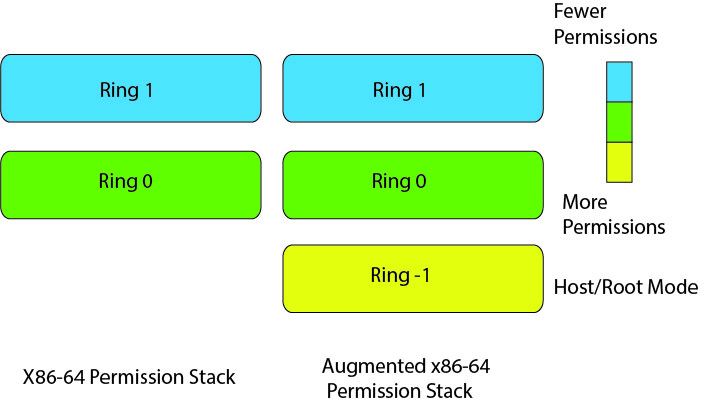
\includegraphics[width=\textwidth]{figures/AugmentedPerm.jpg}
	  \caption{Augmented x86-64 privilege Stack}
\end{figure}

\subsection{Virtualization}

Virtualization itself is not a new concept. It began in the 1960s with the IBM System 360 ~\cite{vleck_ibm_2010}. This system, like most others for the next nearly four decades, used the trap and emulate model. In this model a virtual machine (VM) will proceed unaltered until it reaches an instruction, which it cannot execute due to an insufficient privilege level ~\cite{popek_formal_1974}. The guest operating system then faults to the hypervisor which performs some set of instructions. This set of instructions will then perform an operation with an identical effect to the original instruction. 

In 1974 Popek and Goldberg ~\cite{popek_formal_1974} formalized the conditions, which were sufficient to allow a CPU architecture to support virtualization. To begin they define a Virtual Machine Monitor (VMM) as a piece of software which provides a programming environment which is ``essentially identical'' ~\cite{popek_formal_1974} to the machine being virtualized (fidelity), only causes a minor performance decrease (efficiency), and is in complete control of the resources (resource control or safety).

Popek and Goldberg then seperate CPU instructions into three different classifications.  Privileged instructions are those which will cause a fault if run in user mode (such as the Intel $cli$ ~\cite{_intel_2015} instruction), control sensitive instructions which change the configuration of resources in a system (the Intel $cli$ instruction also falls into this category),  and behavior sensitive instructions whose affects vary based on the configuration of resources (such as the $popd$ ~\cite{_intel_2015} instruction which varies based on privilege level).

With these requirements and definitions acting somewhat as axioms Popek and Goldberg give us two theorems ~\cite{popek_formal_1974}



 \begin{theorem}[Popek Theorem 1]
 \label{Popek I}
 {
 ``For any conventional third generation computer, a virtual machine monitor may be constructed if the set of sensitive instructions for that computer is a subset of the set of privileged instructions'' ~\cite{popek_formal_1974}
 }
 \end{theorem}


\begin{theorem}[Popek Theorem 2]
 \label{Popek II}
 {
 ``A conventional third generation computer is recursively virtualizable if it is virtualizeable and a VMM without any timing dependencies can be constructed for it.'' ~\cite{popek_formal_1974}
 }
 \end{theorem}



The proofs for these theorems can be found in the original work by Popek and Goldberg. The first theorem says that a VMM can only be constructed for an architecture if the sensitive instructions are a proper subset of the privileged instructions and the second says an architecture is not virtualizable if a VMM cannot be constructed for it.  

This model is not appropriate for x86 virtualization however as many of the x86 assembly instructions, such as $popd$~\cite{_intel_2015}(which pops an element off the floating point stack),  are sensitive but not privileged. This violates the conditions required for VMM construction of Popek's first theorem and by extension x86 cannot be virtualized via the trap and emulate method. 

In 1999 VMware patented their techniques for binary translation, which they introduced in 1998~\cite{rosenblum_vmwareas_1999}, allowing the x86 architecture to be virtualized.  In binary translation the hypervisor runs one ring below the guest OS (in Host/Root mode on x86-64).  The translator reads guest memory starting at the instruction pointer (eip/rip) and caches up to 12 instructions (fewer if a terminating instruction is reached) in a Translator Unit (TU). Unprivileged and non-sensitive instructions (such as mov or xor) are translated IDENT (identically) with no changes made. 

Privileged and sensitive instructions however are translated producing Compile Code Fragments (CCF) using non-privileged instructions. Agesen et. al. ~\cite{agesen_evolution_2010} use the $cli$ instruction as an example. The $cli$ instruction clears the interrupt flag on the physical CPU. 
Since the guest VM cannot (and should not ) clear the interrupt flag on the physical CPU the interrupt flag is cleared on the VCPU ($vcpu.flag$) using the $and$ instruction. Once a TU is translated into a CCF it is then run on the CPU. 

This began the boom in x86 virtualization, which was shortly followed by the introduction of Xen in 2003~\cite{barham_xen_2003}, which introduced the paravirtualization method for x86 virtualization. In paravirtualization, like binary translation, the hypervisor runs at Ring 0, the guest OS runs at Ring 1, and user code runs at Ring 3.  Paravirtualization works by using a modified kernel, replacing instructions which will require hypervisor support such as those involving memory Managementment with hypercalls~\cite{barham_xen_2003}.  These hypercalls result in the hypervisor peforming some operations which result in the a state being presented to the VM which from its perspective appears that it has been performed on physical hardware rather than on a VM. This allows the guest to run without any modification to user space code much like trap and emulate and binary translation. This method, however, traditionally requires that a specific kernel be used, which greatly increases the time between versions and makes the virtual environment sensitive to OS changes. As of Linux version 3.0 however the introduction of Paravirt Ops into the Linux kernel has added native paravirtualization support removing this limitation~\cite{_understanding_????}. Due to the nature of paravirtualization we are limited in a practical but not theoretical sense to open source operating systems such as Linux~\cite{_Linux_archive} and BSD~\cite{mckusick_design_2004}.

The 64-bit line of x86 processors was introduced by AMD in 2003 and this line only had 2 level of privilege unlike the 4 in the 32 bit lines. The result was there was no longer room to run a hypervisor, guest OS, and user code each on their own privilege level. In 2006, Intel (VT-x ~\cite{neiger_intel_2006}) and AMD (AMD-V ~\cite{codenamed_pacifica_2005}) both added hardware virtualization to their x86 line of processors. Hardware virtualization adds another layer in the privilege stack below Ring 0 called the Host Mode and Root Mode for Intel and AMD respectively. These are colloquially, though not formally, referred to as Ring -1. A structure called a Virtual Machine Control Block (VMCB) is defined in hardware. This structure holds the list of all instructions to be intercepted. Certain instructions are required to fault by the hardware but others can be added to the VMCB by the hypervisor. This method allows the guest OS to run on Ring 0 of the hardware as it would normally expect to. The guest runs normally until it has to run an instruction which requires a fault (as defined in the VMCB). The instruction which caused the fault is then trapped and handled by the hypervisor. Any operating system can be virtualized in this manner, however it does require special hardware instructions (though those are now available on almost all Intel and AMD CPUs) and the shifts to the Host/Root mode are time consuming and need to be reduced to the smallest number possible to keep the process efficient.

Shortly after the advent of X86 hardware virtualization ~\cite{neiger_intel_2006}~\cite{codenamed_pacifica_2005} the hypervisor KVM (for Kernel Virtual Machine) was introduced by Kivity et al ~\cite{kivity_kvm:_2007} and was included as part of the main line Linux[18] kernel the same year. As part of the Linux kernel KVM is able to reduce some of the code base by incorporating certain aspects of the Linux kernel such as the scheduler in order to handle managing resources of virtual machines.  Throughout this experiment we will be using either Xen or KVM as appropriate. Due to the differing architectures of the two hypervisors there will be some approaches that will work with one and not the other. Where applicable we will comment on why one was chosen for a specific experiment over the other.





\subsection{X86-64 Memory Architecture}\label{x86mem}

Modern commodity CPUs use an architecture known as the Von Neumann Architecture ~\cite{von_neumann_first_1993}.  At the most basic level a computer based on the Von Neumann Architecture consists of a CPU which processed data and instructions, memory, mass storage, and input/output devices.  Due to limitations on the throughput between the different parts of a computer we encounter what's known as the Von Neumann Bottleneck~\cite{von_neumann_first_1993}.  Data on a CPU register is fast to access, RAM is slower, disk drives slower still, and network based storage the slowest available. 

To address this problem CPU cache was introduced. Cache is a small amount of extremely fast RAM which exists on the CPU in order to alleviate, but not eliminate, the Von Neumann Bottleneck.  In a modern X86-64 CPU there are three levels of cache: L1, L2, and L3. L1 is the smallest and fastest with L2 being slightly larger but slower and L3 being even larger and slower. 

On a modern CPU the process of accessing memory begins by checking the Translation Lookaside Buffer (TLB). The TLB is a small amount of cache which holdes virtual address translations in the form of Page Table Entries (PTEs). These entries (discussed further in section \ref{PageTable}) map virtual memory to physical memory. If the entry is in the TLB we have a TLB hit.  If this occurs we look to see if our physical address is in the L1 cache. If this is the case we have an L1 cache cit and the data is loaded into the CPU. If this is not the case we have an L1 cache miss. If this occurs we look to see if our physical address is in the L2 Cache. Again if it is we have an L2 Cache Hit and load our data to the CPU. If an L2 Cache Miss occurs we have to check the L3 Cache. Unlike the L1 and L2 Caches the L3 Cache is shared by all cores on a CPU. If our physical address is in the L3 cache we have an L3 cache hit and our data is given to the CPU. Otherwise it requires looking to see if the data is in DRAM. In the event of a TLB miss a walk of the page table is necessary (~\ref{PageTable}). 
\begin{figure}\label{X86Mem}
	  \centering
	  \includegraphics[width=\textwidth]{figures/X86MemoryHeirarch.jpg}
	  \caption{X86-64 Memory Heirarchy}
\end{figure}

Each of the steps described before contributes to our Average Memory Access Time (AMAT). The formula for computing AMAT is described in equation ~\ref{AMAT}. Where $H_i$ is the time per hit on the some memory element (e.g. Cache or the TLB), $AMP_i$ is the average penalty per miss on that element, and $M_i$ is that a miss will occur on that element. This is summed over all the elements of memory. 

\begin{equation}\label{AMAT}
	AMAT = \sum_{i=0}^{n}{H_i+AMP_i\times M_i}
\end{equation}

\subsection{Virtual Memory and Paging}\label{PageTable}

In a modern programming environment memory is abstracted so that each process sees its physical memory as one contiguous region.  This is a convenient abstraction made possible through virtual memory. In modern x86 and x86-64 virtual memory is provided through a system called paging. In paging memory is broken into segments called pages, which are typically 4kb though larger pages are supported up to 2MB and 1GB for 32-bit and 64-bit x86 respectively. A data structure called the page table is used to map virtual memory that the process sees to physical memory. In the x86 architecture this mapping is handled by hardware known as the Memory Management Unit (MMU). 

The x86-64 processor uses a 4 level paging system to translate virtual addresses to physical addresses when 4kb pages are used and a 48-bit address space. The levels are organized in a tree structure. The CR3 holds location of the page directory for the process. The first 16 bits are unused, next 36 bits are broken into four segments of 9-bits each. The first is called the Page Map Level 4 page (PML4), the next is called the Page Pointers Directory page (PDP), the next is called the Page Directory page (PD), and the final one is called the Page Table page (PT). The remaining 12 bits are for the page offset, which tells us where in the page the memory is located Fig ~\ref{VirtPaging}~\cite{_file:x86_2009}. 

\begin{figure}\label{VirtPaging}
	  \centering
	  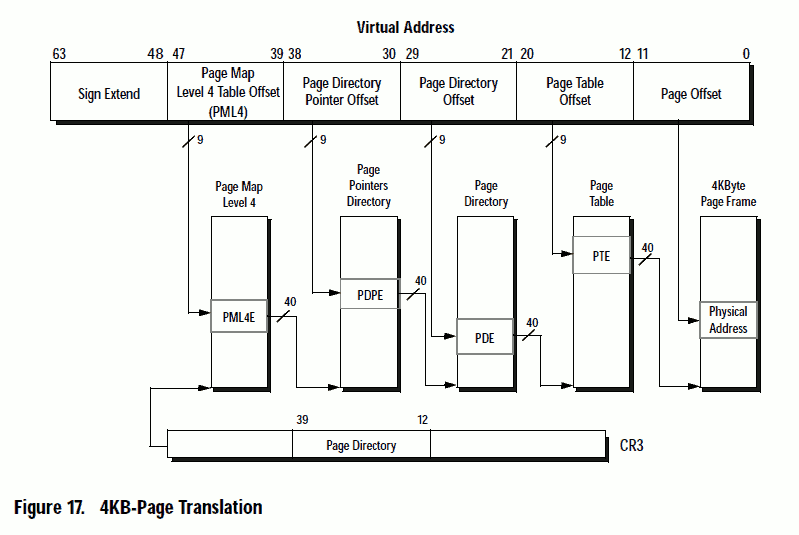
\includegraphics[width=\textwidth]{figures/Orion64BitTranslation.png}
	  \caption{Page Table in x86-64 ~\cite{OrionPaging} }
\end{figure}



\section{Xen}
Xen is a type-1 or ``bare metal'' hypervisor. This means that Xen runs directly on the physical hardware and is not itself hosted in another environment. This is in contrast to a type-2 hypervisor like VMWare Player which is hosted inside a Linux or Windows environment. Administration of Xen and its VMs is done via a special paravirtualized guest called the Dom0. All other guests in Xen can be either paravirtualized or hardware virtualized. For the remainder of this dissertation we will assume all DomU guests (those guests which are not Dom0) are hardware virtualized unless otherwise specified.

\subsection{Xen Virtual Memory Management}

As Xen supports two different types of virtualization it also supports three different kinds of virtual memory management. Traditionally software virtualization uses a shadow paging scheme ~\cite{barham_xen_2003} which keeps an additional ``shadow'' page table. This provides an additional layer of abstraction between the guests and the physical hardware. 

Since paravirtualized guests use hypercalls for sensitive instructions Xen is not required to keep a full shadow page table for its memory management, instead using a technique known as direct-paging. In direct paging guests invoke a hypercall which directly maps their page table entries from virtual memory to physical memory as opposed to the extra paging layer provided in shadow page tables~\cite{barham_xen_2003},  essentially moving control of memory management from the OS to the hypervisor. In this way ultimate control of memory management is transferred from the guest OS to the hypervisor. 


Since hardware virtualized (HVM) guests are not modified in the way that paravirtualized guests are, they do not have the option of this direct-paging technique and instead have the option of either hardware assisted paging (HAP) or shadow paging. HAP uses a technique called Second Level Address Translation (SLAT) Fig ~\ref{SLAT} which is included in Intel processors since the Nehelem line and AMD processors since the Barcelona line. Their technologies are called Extended Page Tables (EPT) and Rapid Virtualization Indexing (RVI) respectively. In SLAT the guest OS still maintains a logical page to physical page mapping (fig 2). However these physical pages are in pseudo pages and do not correspond directly to physical memory. Instead the hypervisor maintains the pseudo physical to machine page (or actual physical page) mapping.  


HVM guests also have the option of using a shadow page table (SPT) similar to that used in VMWare~\cite{rosenblum_vmwareas_1999}.  Like HAP shadow paging works by adding another layer of abstraction to paging. In this model the processes use the software page tables provided by the OS just like they would normally. When a guest OS tries to update a page a shadow page is allocated. This shadow page can be then altered with no constraints. When the page is ready to be moved into the regular page table (i.e. permanent changes have been accepted) references are updated such that they point to the new page rather than the original.

\begin{figure}\label{SLAT}
	  \centering
	  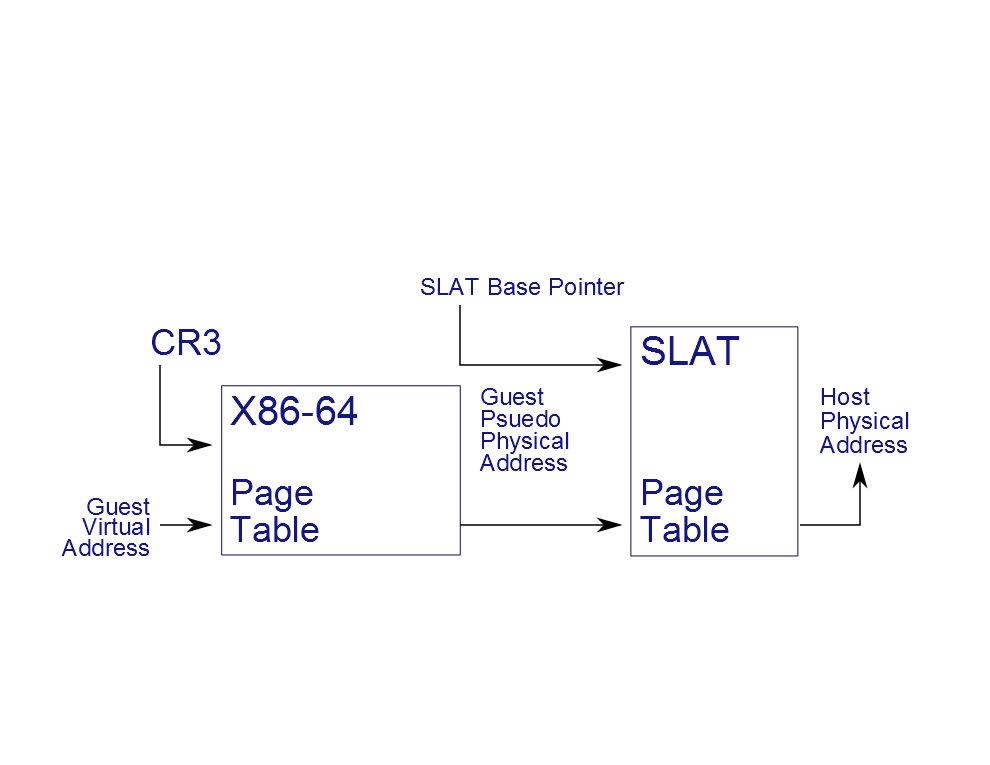
\includegraphics[width=\textwidth]{figures/BM_Graph1.png}
	  \caption{Diagram of Hardware Accelerated Paging using SLAT }
\end{figure}

\section{KVM}

Like Xen, KVM is a type-1 (i.e. Bare Metal) hypervisor. Unlike Xen, which is an independent hypervisor loading up a paravirtualized Linux VM as the administrative unit, KVM is itself integrated into the Linux kernel, which allows the use of a non-virtualized Linux environment for administration (as opposed to the paravirtualized Linux environment used in Xen). As a result of being part of the Linux kernel, KVM is able to use portions of the Linux kernel, for instance KVM uses the Completely Fair Scheduler ~\cite{pabla_completely_2009} used in the kernel to schedule CPU time for VMs. Other functions such as memory management are also done using the internal Linux mechanisms.  

\subsection{KVM Page Merging}

In version 2.6.2 of the Linux Kernel a scheme called Kernel Samepage Merging ~\cite{arcangeli_increasing_2009} was introduced. In this scheme pages which are identical among processes are merged in order to save memory. To accomplish this processes which may be candidates for merging register with the kernel. The kernel then scans the registered areas of virtual memory by taking the hash of those pages. Pages which have unique hashes are skipped for the remainder of the scan, while pages which have the same hashes are then checked byte by byte to ensure they are identical and avoid hash collision. Identical pages are then merged by first marking all page table entries where page occurs as unwriteable. Next all page table entries which refer to that page are updated so they point to only one instance of the page. The remaining unmerged copies of the merged page are then freed and a final direct memory comparison is made to ensure that the pages have not changed. These merged pages can only remain merged so long as the processes or VMs using them are only reading from them. To address this KVM uses a Copy-On-Write (COW) scheme. With this technique pages remain merged until one guests attempts to write to it. When that occurs a copy of the page is made for that guest and the remaining guests continue to use the merged page. 




\section{Virtual Machine Introspection}

Garfinkle and Rosenblum ~\cite{garfinkel_virtual_2003} introduced Virtual Machine Introspection (VMI) in 2003. In VMI the state of a running VM is interpreted by some external entity, usually either another VM or by the host system. To accomplish this memory is mapped or copied from the target VM to the VMI program. Memory is then interpreted to determine some portion of the internal state of the target VM. While the original work was used for intrusion detection a number of other applications have emerged in the years following. 

Memory outside of a given context has no intrinsic meaning,  only inside a given context or process does it have meaning. As such memory in a guest OS has no meaning outside of that guest. This problem is known as the semantic gap. The typical way to solve the problem ~\cite{garfinkel_virtual_2003} ~\cite{hay_forensics_2008} is to use a template approach for each individual OS. In this approach certain areas of memory are marked as being where certain structures in kernel memory are located.  That way a VMI agent can look for the relevant areas in memory and interpret them at run time.  The process of determining the location of these kernel structures can be time consuming, error prone, and must be repeated for each version of a running kernel. Work is being done to address the problem of the semantic gap and is addressed later in this dissertation. 

At its most fundamental level VMI represents a mapping of memory from the guest to an area outside of the guest (be it another VM as in the case of Xen or an administrative Linux OS as in the case of KVM). In this case we can study one method for VMI without losing generality. For our experiments we will use VMITools ~\cite{payne_vmitools_2014}. It is an open source framework to allow easy development of VMI applications, supports Linux and KVM, and has appeared in a number of works on VMI (though in some of these works it appeared under its former title XenAccess) ~\cite{dolan-gavitt_leveraging_2011, zhao_vrfps:_2009, lengyel_virtual_2012, weingartner_promox:_2009, marken_using_2014}.

\section{Virtual Machine Introspection Literature}

Gu et. al. ~\cite{gu_process_2011-1} introduced a scheme for active VMI. In this scheme for VMI a process is injected from the hypervisor to the guest VM. This process is hidden inside an innocuous process already running inside the VM. These processes are called the implanted process and the victim process respectively and are both chosen by the host administrator at runtime. When the victim process is scheduled to be run, the hypervisor captures the context switch. The implanted process the replaces the victim process. To accomplish this the relevant instruction pointers are changed as well as the relevant stack pointers etc. When the OS resumes to continue the context switch the implanted process is run in place of the victim process. Once the implanted process has completed or the hypervisor determines it is time to switch the context back the contexts are switched and the victim process runs is executed normally. 

In the initial experiments ltrace, a program to scan the libraries called by a process, is implemented as the implanted process. This allows them to implant ltrace into a running VM and are able to trace the library calls of selected processes. While this does accomplish some of the goals of conventional VMI it can also be unusable for applications such as digital forensics in which a VM must remain unaltered in any capacity in order to be of use in a courtroom setting. 

Dolann-Gavitt et al introduce a system called Virtuoso ~\cite{dolan-gavitt_virtuoso:_2011} which is aimed at bridging the semantic gap. The execution of Virtuoso is broken into three phases: The training phase, the analysis phase, and the runtime phase. 

In the training phase Virtuoso attempts to gain information about the guest. Inside the guest a program must be written to access the information desired. For instance if one were trying to write a VMI program to access the Process Identifiers (PIDs) then one would write an in guest program which would access the process IDs. This program would then be run repeatedly and each time it was run a syscall trace (such as with Linux strace) would be taken of that program.  After running this program repeatedly an extensive list of execution paths would be generated. Using this combination of execution paths the analysis phase can begin. 

The collection of syscall traces, while it does contain the necessary execution paths, also contains a great deal of extraneous noise. This is because the system trace follows the entire execution through the system not just the relevant information. Parts of the trace, which are known a priori to be unnecessary such as hardware interrupts or memory management, are thrown out immediately. Then a dynamic data slice ~\cite{agrawal_dynamic_1990} is then done. There slices are merged into a unified program which can be turned from an in guest program to an out-of-guest program. 

The translated code cannot be run directly on the host. So Virtuoso creates a runtime environment for the translated code. The run time environment is installed on the host machine and has the ability to run the translated code. This gives the code created by Virtuoso an appropriate context from which to access the VM resources (e.g. CPU registers or main memory) in a read-only manner.

While Virtuoso does make significant progress in bridging the semantic gap it does not change the fundamental nature of introspection. The tools generated by Virtuoso still simply read and interpret memory from the guest, which means that our study will still apply to virtuoso without having to directly address virtuoso. 


Like Virtuoso, Fu and Lin ~\cite{fu_bridging_2013} make an attempt at bridging the semantic gap and automatically generating VMI utilities.  The process begins with an untrusted target VM (called the product-VM) and a secure trusted VM (called the secure-VM). Three techniques are then used to extract information from the product VM. These are syscall execution context identification, redirectable data identification, and kernel data re-direction. 

The context being executed is identified using a stack to keep track of times iret  and int are called. Global kernel data is then identified using an adapted form of taint analysis. With the relevant information located and the contexts identified they are then able to redirect the kernel information between the product-VM and the secure-VM. This allows native system monitoring utilities to be run on the secure-VM as VMI targeting the product-VM unaltered. 

In their results many of the native Linux utilities such as lsmod ~\cite{kerrisk_lsmod8_2014} gave identical results as if they were inside the product-VM itself. However certain utilities like date ~\cite{mackenzie_date1_????} and ps~\cite{lankester_ps1_????} produce similar but not identical results. This was found to be due to the timing of the snapshots they were using for the analysis as certain programs are quite time sensitive. While this has approached an automatic bridge for the semantic gap this work is still reliant on semantic information about system calling conventions and can be altered if they are changed between kernels. This seems like a promising tool to use for VMI however as of this publication the source code has not yet been released for use by the public, so it will remain unstudied in this work. 


\subsection{Uses for Virtual Machine Introspection}
In this section we will discuss current uses for VMI especially as they related to information assurance and security. 

In Crawford and Peterson ~\cite{crawford_insider_2013} VMI is leveraged to address the insider threat problem.  The insider threat problem is the situation that occurs when current or past members of an organization have both malicious intent and legitimate access to a system or systems ~\cite{rushby_critical_1994}. To accomplish their goal they break their approach into four steps: Development of a taxonomy of malicious insider behavior, development of a taxonomy of VMI observables, malicious insider detection, and data validation. 

To develop a taxonomy they began by setting up a number of possible high-level uses cases. The activities identified in this taxonomy are printing activity, disabling defensive tools (e.g. anti virus), abusing removable media (e.g. putting sensitive information onto a flash drive), sudden change in employee behavior, use of remote access, and strange clipboard activity. Once they determine major uses cases they wish to look for they decompose each scenario into individual observable attacks and each attack is broken down into seven areas of analysis. These areas are the attacker (who is doing something or can do something), which tools are used, which vulnerabilities are used, what actions are taken in order to achieve the desired effect, which systems are targeted, what the result of this unauthorized attack is, and what the objective of that result is. Using this taxonomy they can break many insider threat problems into simple terms. 

The next step is to determine which parts of a system can be observed by VMI. The observables consist of ``registry information, hexadecimal patterns, and clipboard information.'' Each of the potential malicious activities is performed while the observables are being monitored by VMI. If those observable areas create signature patterns then they can be used to identify the insider threat actions from VMI. The relevant observables are provided in the work from Crawford and Peterson ~\cite{crawford_insider_2013}. 

The third step is essentially the experiment portion of the paper. During the experiment VMI is used as well as Windows event logs. VMI and Windows event logs are analyzed while certain potentially malicious operations described earlier were performed. The experiment recorded which actions set showed as being malicious and which ones did not. 

The final step is the analysis phase. For each attack in the scope of the research they perform it manually several times to determine if their tools developed from the third phase are capable of detecting it. Their results showed that they were able to detect 18 different types of insider attacks. They report a high false positive rate though they don’t give the specific rate of either detection or false positives. The authors indicate that while this work shows potential more work needs to be done on determining which observables correlate to which observables can indicate attacks in order to increase the accuracy of their detection. 

Harrison et al ~\cite{harrison_constructing_2012} have proposed using VMI combined with the related yet distinct field of Forensic Memory Analysis (FMA). Harrison’s goal is to put together an entirely out-of-band passive sensor to monitor for malicious software such as kernel rootkits. Like all current VMI approaches FMA is adversely affected by the semantic gap. In order to address this situation a file system was built using FUSE~\cite{rajgarhia_performance_2010}, which translated the page table such that the memory of the VM was able to be read as one contiguous “file”. The volatility framework for FMA is then used in order to analyze the contents of the memory. A rule learning algorithm called IREP++ ~\cite{dain_irep_2004} is used as a classifier in order determine if any intrusions are made into the system (such as kernel rootkits) were made and the results are logged into a postreSQL database. This is an interesting approach to side-stepping rather than attempting to directly solve the semantic gap. Volatility however like many VMI approaches still relies on a priori knowledge of the location of data structures inside the kernel which may leave this approach vulnerable to attacks which manipulate those structures. 

Hay and Nance ~\cite{hay_circumventing_2012} developed a method for using VMI to read the plaintext for encrypted data with the VIX tool suite~\cite{hay_forensics_2008}.  While direct attacks on modern cryptographic systems such as AES is generally computationally intractable three basic facts are noted: Before being encrypted cipher text exists in an unencrypted form, after being decrypted cipher text exists in an unencrypted form, and encryption requires that somewhere on the system cryptographic keys exist. To take advantage of the first two it is a simple matter of observing the state of VM while the plaintext is in memory.  The third requires two steps; recover the key while it exists in memory and use that key as to recover the plaintext using the appropriate decryption algorithm. This use of VMI is an instance of security software which has great use for law enforcement and intelligence agencies as well as great potential to be misused as well.

\section{Information Leakage and Side Channel Attacks}

In this section we discuss the current state of research into information leakage and side channel attacks.

\subsection{Side Channel Attacks}
While a number of side-channel attacks have been explored in the past~\cite{yu_approach_2013,ristenpart_hey_2009, zhang_cross-vm_2012} a formal model of the information leakage due to these attacks was first introduced by Demme et al ~\cite{demme2012side}. Demme introduces the Side-channel Vulnerability Factor (SVF) in order to determine exactly how vulnerable a certain cross-channel attack makes a system. 

The SFV begins with an oracle, which contains the truth about the execution of the victim. The side-channel produces the information that an attacker is able to measure. An example of an oracle could be number of accesses to a certain page and the side-channel could be the average power consumption on the host. A perfect side-channel would be able to trace the oracle trace directly. The SVF also requires a distance metric. The distance metric could vary from problem to problem. For instance if the data were represented by vectors the Euclidean or Manhattan distances could be used. 


Next they establish a similarity matrix for both the oracle and side-channel traces. These similarity matrices are necessary since oracle and side-channel are by their very nature measuring different things (such as pages accesses versus cache access time).  

Next they establish a similarity matrix for both the oracle and side-channel traces. These similarity matrices are necessary since oracle and side-channel are by their very nature measuring different things (such as pages accesses versus cache access time).  The similarity matrix M is defined as being of length $S$ and size $|S|^2$.  Each element of $M$ is defined as 




\begin{equation}\label{eqn:simMatrix}
M(i,j) =  
		\begin{cases}
			D(S_i, S_j) & if \ i  >  j \\
			0 & otherwise \\
		  \end{cases}
\end{equation}

where $D$ is our distance function.  This creates a triangular matrix with no diagonal. The matrices are compared elementwise and the Pearson correlation coefficient between the two is computed. The further from 0 the Pearson Correlation Coefficient is the more information is leaked through a side channel. A coefficient of 1 will mean the channel is perfectly transparent and a coefficient of 0 will mean that the channel is totally opaque. 

This SFV will be able to provide us with a measure to tell how our different approaches to information leakage will be relative to each other. As well as a measure of how much information leaks from VMI relative to other types of information.

\subsection{Determining Co-Residency} 
Ristenpart et al ~\cite{ristenpart_hey_2009} introduced a scheme for determining co-residence by measuring the load on the cache. In their paper they did a variant on the cache-probe technique which relies on the architecture of the x86 cache. It begins by allocating a buffer $B$ of size $b$ bytes, where $s$ is the size of the cache line.  Their initial attack is broken into three pieces

\begin{enumerate}
	\item Prime: Read $B$ at $s$ byte offsets. (Ensuring that $B$ is in cache)
	\item Trigger: Wait until the number of CPU cycles passed jumps by some large value (to determine if the VM has been interrupted by the Xen credit scheduler)
	\item Probe: Measure how long it takes to read $B$.
\end{enumerate}

In step 3 $B$ is accessed in pseudorandom order in order to prevent the hardware pre-fetcher from hiding the latency. These latencies correlate strongly with use of cache during the trigger step. However due to Xen s scheduling algorithm this is not quite enough to measure the cache latency. For that they expand the prime-probe attack even further to the following.

\begin{enumerate}
	\item Allocate $B$ contiguous bytes.
	\item Sleep briefly (to build up credits with Xen's scheduler)
	\item Prime: Read all of $B$ to make sure it's fully cached
	\item Trigger: Busy loop until the number of CPU cycles jumps by a large value
	\item Probe: Measure how long it takes to read $B$
\end{enumerate}

Through this load measurement and comparison to VMs running known services they are able to determine which VMs are co-resident. 

Zhang et al ~\cite{zhang_cross-vm_2012} put forth another scheme for determining co-residency of VMs on the Amazon EC2 cloud ~\cite{_aws_EC2_2014} by measuring the load on the cache. In this attack we consider two entities $U$ and $V$ each of which share a common cache. Then a similar prime-probe method as above is used though it is modified to function as follows

\begin{enumerate}
	\item Prime - $U$ fills a cache set by reading a region from its own memory
	\item Idle - $U$ waits for a specified interval during which the cache is used by $V$
	\item Probe - $U$ times the reading of the same cache set in order to learn of $V$`s activities
\end{enumerate}


In their initial trials the VM represented by $U$ attempted to determine if $V$ was co-resident by running one prime-probe trial and averaging the time across all cache sets. If this time was below a certain threshold a foe-absent classification was issued and if it was below that threshold a foe-present classification was issued. This proved to be extremely unreliable for two primary reasons: The Xen scheduler balances load by shifting VMs to different cores which may not share physical caches and because friendly VM activity on other cores , especially IO activity, will cause activity in the Dom0 which will introduce significant noise into the cache. In order to deal with this high level of noise a multi-probe classifier was implemented. In this classifier they looked at the results of 2000 prime-probe trials and noticed a pattern appearing to be two overlapping normal distributions. They then use these statistics to determine the classification. 

In Owens and Wang ~\cite{owens_non-interactive_2011} a scheme using the memory de-duplication techniques provided by commodity hypervisors (specifically ESXi ~\cite{chaubal_architecture_2008} in this case). They begin by assuming that an attacker can instantiate VMs in the same environment as the targeted VM and that the attackers has root control over any VMs it instantiates. Further they assume the standard 4kb pages size. To begin their procedure they first determine which pages are unique to a specific OS version and are present in all versions of that OS. They must also determine which of those pages are relevant to their analysis, for example a memory dump of Windows XP SP3 contains 59,238 pages of zeros~\cite{owens_non-interactive_2011} These are not useful to the analysis. They are then able to determine which pages are signature pages for each OS. 

At this point they take advantage of the de-duplication mechanism in ESXi. When ESXi writes a non de-duplicated page a simple write is performed. However when writing to a de-duplicated page a copy is made of that page and then it can be written to. The memory allocation and copy of the new page takes a measurable level of overhead. While there is overhead from the copy it can also be easily confused with the computational overhead from reading a page which has been swapped out having not been used recently. To handle this a read operation is performed on the signature page immediately before attempting an OS fingerprinting operation. They are then able to plot the timing results and can demonstrate which OS is being run on the host. 

Xiao et al ~\cite{xiao_security_2013} explored the implications of memory de-duplication on security in a more general sense by putting together both a reliable attack using this technique and a reliable defense against similar techniques. For their offensive approach Xiao shows that one can transmit data between two co-located VMs using the memory de-duplication. 

They begin with two co-located VMs with a hypervisor which uses memory de-duplication. Each VM creates a number of identical pages. This can be easily accomplished by reading an identical file into memory. Then the sender encodes the information which it wants to transmit to the receiver. It does so by writing to certain pages and not to others. The sender and the receiver then sleep for some amount of time to allow the pages to be merged by the hypervisor`s memory de-duplication mechanism. The receiver then writes to each of the pages and times the amount of time it takes to make these changes. Because of the Copy-On-Write(COW) nature of these systems it takes slightly longer to write to a de-duplicated pages as it makes a copy before writing to it. In this way memory can be encoded into bits. A page which has been merged representing a 0 and a page which has not representing a 1. So if both VMs allocate 8 pages in this manner and wishes to transmit 10011001 the sender would alter pages 1,4, 5, and 8 so they would not merge. 

In addition to transmission they were also able to determine that one was in a virtualized environment using the artifacts of memory de-duplication. A file is read into memory and then all pages in memory are written to and the write access times are recorded. Then the file is read in its entirety into two different memory locations. Since every page of the file has an exact duplicate in memory the hypervisor’s de-duplication mechanism (if present and virtualized) is likely to merge the pages after an appropriate amount of time. Then one of the identical pages can be written to, if the environment is virtualized with memory de-duplication then the write access time will be significantly higher than the original write access times due to COW. 



As a defensive mechanism agaisnt these attacks Xiao suggests a kernel runtime integrity scheme.  There several hypervisor based mechanisms for determining the presence of kernel rootkits running in guests ~\cite{butler_windows_2005}~\cite{hoglund_*real*_1999}. These all require extensive knowledge of the kernel in order to bridge the semantic gap. Xiao proposes examining the kernel for the sections of data, such as the syscall table, which are meant to be read-only. Inside the kernel binary read only data is designated by the .rodata section. This data is copied and read by a C program inside which holds an exact copy of the read only kernel data in memory. 

A statistic gathered by Linux called the Proportional Set Size (PSS) is then used in order to determine whether kernel integrity has been threatened. The PSS value is the number of unique pages and the weighted number of the duplicated pages a process has. For instance a process with 100 unique pages and 100 duplicated pages would have a PSS of 150 ~\cite{xiao_security_2013}. This value is stored in the file /proc/\$pid/smaps. A simple shell script can then determine if the PSS value has increased significantly to determine if kernel integrity has been violated. 

These side-channels are directly applicable to determining whether or not a VM is being monitored by VMI. Linux uses a technique called Kernel Same Page Merging (KSM) to reduce memory commitment from processes in a manner similar to how ESXi de-duplicates pages for VMs. The KVM hypervisor treats all VMs as if they are Linux processes. As a result it is possible that identical pages between a VM and some Linux process can be merged thus causing a measurable delay when these pages are written to. If the VMI program happens to hold a page identical to one in a guest VM then it's possible that the VMI process can be detected through this delay. 

Zhang et al ~\cite{zhang_cross-vm_2012} introduced a scheme for reading cryptographic keys used by another VM sharing the same physical hardware and hypervisor. A similar prime-probe technique to was used, but this time specifically used on the instruction cache (icache) as opposed to the data cache (dcache). It does so with the standard icache technique introduced by Aciicmez ~\cite{aciiamez_yet_2007}. A icache line is loaded with nops and then filled again with nops and the time difference between the two is noted. Further steps are needed however, as information from another VM is being sought the Xen scheduler has to be taken into account. To handle this interprocessor interrupts (IPIs) are used. In symmetric multiprocessing (SMP) systems processors are allowed to interrupt each other or even themselves through an IPI. To make sure the attacking VCPU has precedence another VCPU (called the interrupting VCPU or IVCPU) runs in a continual loop sending IPIs to the attacking VCPU.

This attack searches for instructions which are a square, a multiply, or a modulus-reduce instruction. In order to do so they use multiclass support vector machine[68] to pick out when these instructions are being used. While this is fairly good at picking out instructions the SVM is subject to the hardware and software noise introduced by the system (things such as TLB misses, or context switches.) To handle this hidden markov models ~\cite{bishop_pattern_2006} are used to filter the noise. This allows them to determine the cryptographic key in as little as 40,000-50,000 brute force attempts. While this may seem like a great deal we keep in mind that 50,000 brute force attempts will take less than 1s on commodity hardware making this a reasonably effective attack. 

These previous works have been directed almost entirely at exploring side-channel attacks aimed at the hypervisor layer. Bates et al ~\cite{bates_detecting_2012} take a lower level approach and investigate whether co-residency of one or more VMs on a hypervisor can be determined via active traffic analysis techniques. They begin by assuming that they are on a normal cloud instance such as EC2~\cite{_aws_EC2_2014} that has been patched against previous co-residency attacks ~\cite{zhang_homealone:_2011}~\cite{ristenpart_hey_2009}. 

\begin{figure}\label{BatesNetworkThing}
	  \centering
	  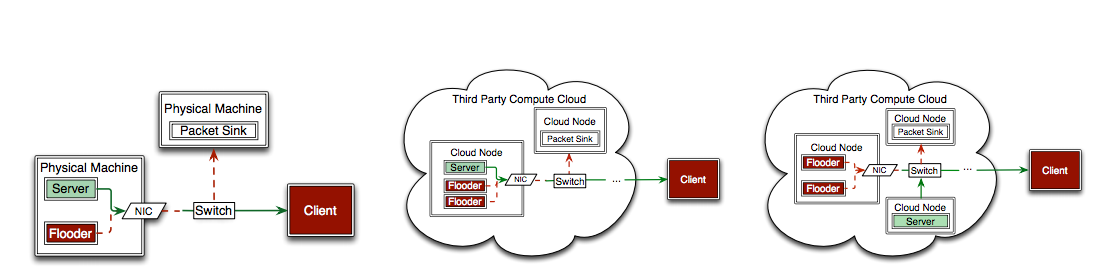
\includegraphics[width=\textwidth]{figures/batesNetwork.png}
	  \caption{Topologies used in active traffic colocation test from Bates et. al. ~\cite{bates_detecting_2012}
	  (left) local test system 	(center) successful co-location   (right) failed co-location }
\end{figure}



Their attack then creates a large number of instances on that cloud service, which they term flooders. Each flooder announces its presence to an external machine called the client. Another instance created in the cloud is called the server. Upon receiving a signal from the server the client sends signals out to the flooders, at which point the flooders begin to send outbound traffic on their machines physical interface to a packet sink which is not the client. This outbound traffic causes a delay in the server flow. 

These delays in server flow form a watermark in the signal from the client and the server. The network flow between the client and server can be given by $T$ and divided into $n$ segments of $t_i$. Watermarks of this kind require two different levels of packet delay to encode their signal represented by $\pm d$. Since negative delays are not possible in this environment they take no delay to represent $-d$ and a delay to represent $+d$. Using this scheme they are able to encode bit values using $-d$ as a 0 and $+d$ as a 1. 

Due to the nature of virtualization and network traffic in general a certain amount of noise can affect the signal. These can come from sources such as network congestion or hypervisor scheduling (as described above in the Xen Credit Scheduler for instance.) When the client receives the signal a Kolmogorov-Smirnov(KS)~\cite{pettitt_kolmogorov-smirnov_1977} test is done for independence. If a signal is embedded in the traffic flow it will demonstrate a different discrete distribution from one without a signal. With the KS test they are able to determine a signal's independence with a 95\% confidence. 

This attack is interesting in that it operates at the hardware layer rather than at the hypervisor layer. It is possible that VMI targeted at the network stack of a VM (such as the VIX ifconfig ~\cite{hay_forensics_2008} ) could cause a change in the delay, which could be detected in the traffic. However this delay is unlikely to be substantial or consistent enough to useful to detect information leakage from VMI.

\subsection{Detection and Defense Against Attacks}

Martin et al ~\cite{martin2012timewarp} introduced a scheme to protect against micro-architectural attacks by obscuring the way the rdtsc instruction works. Micro-architectural attacks such as the cache timing attacks described above ~\cite{zhang_cross-vm_2012,ristenpart_hey_2009,zhang_homealone:_2011} rely on precise timing of micro-architectural events in order to gather their information. Martin proposes a scheme by which they add two delays to the rtdsc counter. One, called the real offset, delays the execution of the rdtsc instruction. The other, called the apparent offset, which adds a random delay to the end of the rdtsc instruction. These delays can turned off in the OS so that system critical portions of the OS such as the scheduler are not interfered with.  While this can be quite effective against certain types of attacks like those listed above it can be easily worked around if an attacker can gain kernel access (for example through a kernel module) and gives their malicious process rights to use the unaltered scheduler. While this may pose a challenge for some side-channel attacks their threat model differs from ours significantly enough that it poses no hindrance.

\section{VMI and Kernel Attack Papers}

Bahram et al ~\cite{bahram_dksm:_2010} introduced a scheme to subvert VMI through Direct Kernel Structure Manipulation (DKSM) also known as direct kernel object manipulation (DKOM). In this scheme the data structures which store information, such as the list of processes, are manipulated in such a way as to attack the semantic gap. 

The way most VMI implementations are implemented a template based scheme is used to solve the problem of the semantic gap. For each kernel known addresses, such as the start of the task list, are fetched on the assumption that their address and composition are invariant. The DKSM attacks this assumption. 

Bahram et al use three different designs for their DKSM attack: a syntax based manipulation, a semantic based manipulation, and a hybrid scheme. The syntax based attacks take advantage of the fact that some fields in the kernel data structures are not used by the OS. An unused field is removed thus changing the template used by the VMI implementation and rendering its output inaccurate.  In the semantic based scheme fields in some data structure of the same length and similar type are swapped so that their order is reversed. This has the same effect rendering the template used by the VMI implementation useless. The hybrid scheme is a combination of the two where fields are removed and rearranged. 

The implementations of these schemes tested are the direct scheme, and the shadow scheme. A third, the return scheme, is discussed but not implemented. The direct scheme manipulates the structures directly using a loadable kernel module. This method had the advantage of being comparably simple to implement but is easily detectable by VMI tools which choose to measure the kernel integrity making it somewhat impractical. 

The shadow scheme begins by taking advantage of the fact that on commodity x86 processors data and code have separate caches specifically the icache and the dcache. As there is a data cache and an instruction cache there is also a data and instruction Translation Lookaside Buffer (DTLB and ITLB respectively) which will be the target of this attack. 

The ITLB is invalidated at some address (pte) causing that page entry to be ejected from the ITLB. A page, located at address pte, which contains the instructions for the DKSM attack called a ``shadow page'', then replaces the page that was ejected. The global bit on the shadow page is marked to prevent it from being forced out of the ITLB due to TLB pressure from context switches. At the end of the DKSM code in the shadow page is a jmp instruction which jumps to the location of the previously invalidated code. This has two functions: First it loads the page into the icache and the ITLB and secondly it returns control flow back to the original code. This scheme is far stealthier than the direct scheme described above, however it is also far more complicated to implement. Both implementations above are reliant on a modified version of the hypervisor (specifically QEMU/KVM ~\cite{bellard_qemu_2005} in this case) in order to trace memory to learn which fields of a kernel structure are accessed by which functions. This makes these attacks impractical outside of a laboratory environment and the first to take in improving them would be to rectify this short-coming by setting up a way to analyze kernel structure access internally. Further this paper only explored the ``spatial'' aspect of introspection. That where the structures are in memory and ignored the time based aspect of introspection which takes a finite amount of time to create its view and thus is potentially vulnerable to timing based attacks~\cite{bahram_dksm:_2010}. 
